\section{Model Formulations}
\label{chap:physmodel}
%We focus on the melt migration beneath a mid-ocean ridge using a viscous Darcy-Stokes coupled flow model.
%The static mechanics model based on the mixture theory mixing with the porosity parameter $\phi$, 
%which captures the physics of a slowly creeping solid matrix, melt flow through porous media and compaction 
%/ollowing the discussion in~\cite{ctx23979187210006011},~\cite{MagmaPhysics} and~\cite{Fowler01031984}. 
%The static mechanics model is coupled with
%the transport equations of energy and chemical species and thus evolving the system in time. 
%We assume that the system achieve thermodynamical equilibrium at each time step and therefore a phase diagram 
%can be used to compute the thermodynamic status.
We investigate melt migration beneath a mid-ocean ridge using a viscous Darcy–Stokes coupled flow model
%~\cite{ctx23979187210006011},~\cite{MagmaPhysics} and~\cite{Fowler01031984}. 
~\cite{ctx23979187210006011, MagmaPhysics, Fowler01031984}. 
The governing equations are derived from mixture theory and formulated in terms of the porosity, 
$\phi$, which characterizes the volume fraction of melt.
This framework captures the essential physics of a slowly deforming solid matrix, melt percolation through 
a porous medium, and compaction processes.

The mechanical model is coupled with transport equations for energy ~\cite{MagmaDynamicsEnthalpyMethod} 
and chemical species~\cite{GeochemicalConsequence}, resulting in a 
fully time-dependent system. At each time step, we assume local thermodynamic equilibrium, allowing the 
thermodynamic state to be determined from an appropriate phase diagram.

\subsection{Static Flow Model}
%We first write the conservation of mass and momentum of this two-phase mixture based on the 
%Boussinesq approximation disregarding the density difference between the two phases.
%The continuity equation for the two-phase mixture can be written as
We begin by formulating the conservation laws for mass and momentum of the two-phase mixture under the 
Boussinesq approximation, neglecting density differences between the solid and liquid phases except the
gravitational force term. 
The continuity equation for the mixture is given by
\begin{equation}
		  \label{eq:continuity}
		  %\nabla \cdot (\phi\mathbf{v}_l + (1-\phi)\mathbf{v}_s) = 0,
		  \nabla \cdot \overline{\mathbf{v}} = 0,
\end{equation}
where the mixture velocity $\overline{\mathbf{v}} = \phi\mathbf{v}_l + (1-\phi)\mathbf{v}_s$.
%$\mathbf{v}_l$ and $\mathbf{v}_s$ are the liquid and the solid velocities. We use subscripts
%$l$ and $s$ to refer to the quantities associated with the molten liquid magama and the solid matrix. 
Here, $\mathbf{v}_l$ and $\mathbf{v}_s$
denote the velocities of the liquid and solid phases, respectively, and 
$phi$ represents the porosity. Throughout this work, subscripts 
$l$ and $s$ refer to quantities associated with the liquid (magma) and the solid matrix, respectively.

Conservation of momentum for this slowly creeping solid matrix under the assumption of 
low reynolds number can be 
written in terms of the deviatoric stress of the mixture 
\begin{equation}
		  \label{eq:stokes}
		  \nabla\bar p - \nabla \cdot \pmb{\tau}(\mathbf{v}_s) + \overline{\rho}\mathbf{g}= 0,
\end{equation}
where the deviatoric stress of the solid is
\begin{equation}\label{eq:deviatoricstress}
		  \pmb{\tau}(\mathbf{v}_s)
		  = 2\mu_s\phi_s\big(\mathcal{D} \mathbf{v}_s - \tfrac{1}{3}\nabla \cdot \mathbf{v}_s \mathbf{I}\big),
\end{equation}
and $\mathcal{D} \mathbf{v}_s=\frac{1}{2}(\nabla\mathbf{v}_s + \nabla\mathbf{v}_s^T)$ is the symmetric gradient.

The mixture conservation equations~\eqref{eq:continuity} 
and~\eqref{eq:stokes} are insufficient to simultaneously
determine the individual velocities and pressures. To close the system, additional 
constitutive relationships are required to describe the relative behavior of the liquid 
phase within the porous medium.

The relative motion between the molten magma and the deformable solid framework is modeled using 
a Darcy-type law, which characterizes melt segregation driven by pressure gradients and buoyancy 
forces within the porous medium:
\begin{equation}
		  \label{eq:darcy}
		  \phi (\mathbf{v}_l - \mathbf{v}_s)
		  + \frac{k_{\phi}}{\mu_l}(\nabla p_l - \rho_f\mathbf{g})
	    = 0.
\end{equation}
We define the relative permeability 
$k_{\phi} = k_0 \phi^{2+2\Theta}$ with a constant parameter
$\Theta \in [0,1/2]$. 
%This equation shows that the melt segregation
%is controlled by the pressure difference between the molten magma and 
%the porous solid matrix and the relative permeability.~\cite{SIM2020106486} 
%discussed how varying the intrinsic permeability
%would affect the melt segregation pattern under the mid ocean ridge.
This relation indicates that melt segregation is regulated by the relative permeability 
of the porous medium.
Variations in intrinsic permeability $k_0$ can significantly modify melt migration structures 
beneath mid-ocean ridges as well~\cite{SIM2020106486}.
%This relation indicates that melt segregation is governed by the pressure difference between the 
%molten magma and the solid matrix, as well as by the permeability of the porous medium.
%When the liquid pressure exceeds the solid pressure, the solid matrix undergoes expansion.
%Conversely, compaction occurs when the liquid pressure is lower than the solid pressure.
%Variations in intrinsic permeability can significantly modify melt migration structures 
%beneath mid-ocean ridges as well~\cite{SIM2020106486}.

%An unique and essential relationship connecting pressure difference and 
%the divergence of the solid matrix is compaction in the 
%context of mantle dynamics.
%\cite{MagmaPhysics} popularized the concept of
%compaction viscosity and relating the term to the stress balance in a partially
%molten system.
%\cite{TwoPhaseModelCompaction} extended this formulation by incorporating 
%surface tension effects. 
%\cite{Compactioninamantlewithaverysmallmelt} further examined compaction behavior 
%in the limit of infinitesimally small porosity.
Another fundamental constitutive relation in mantle dynamics links the pressure difference 
between the liquid and solid phases to the volumetric deformation of the solid matrix
in a partially molten system~\cite{MagmaPhysics}%through compaction
\begin{equation}\label{eq:compactionviscosity}
		  \xi_{\phi}\nabla \cdot \mathbf{v}_s  =p_l - p_s, 
\end{equation}
where $\xi_{\phi}$ is often referred to as bulk viscosity or compaction viscosity. 
When the liquid pressure exceeds the solid pressure, the solid matrix undergoes expansion.
Conversely, compaction occurs when the liquid pressure is lower than the solid pressure.

We approximate the compaction
viscosity $\xi_{\phi_l}$ 
using a simplified constitutive relationship~\cite{PartialMeltinginUpwellingMantleColumn,MagmaDynamicsEnthalpyMethod},
\begin{equation}\label{eq:bulkviscosity}
		  \xi_{\phi_l} = \frac{\mu_s}{\phi_l^m}.
\end{equation}
In our model, we set $m = 1$. 
%The singularity introduced when $\phi \rightarrow 0$ can be avoided 
%using the scaled formulation~\cite{DegenerateDarcy}.
This equation emphasize the fact that increasing melting production facilitates the compaction of the
solid phase, while in the limit of no melting ($\phi_l = 0$), 
compaction is entirely eliminated.

%We first define the pressure potential
%\begin{equation}
%		  \label{eq:ppotential}
%		  q = p - \rho g h
%\end{equation}

%We focus on the following full static flow mechanical system,
%\begin{alignat}{2}
%    \label{eq:darcy}
%		  &\phi_l (\mathbf{v}_l - \mathbf{v}_s)
%		  + \frac{k_{\phi_l}}{\mu_l}(\nabla p_l - \rho_f\mathbf{g})
%	    &&= 0,\\
%	\label{eq:continuous}
%		  &\nabla \cdot (\phi_l\mathbf{v}_l + \phi_s\mathbf{v}_s) &&=0,\\
%	\label{eq:stokes}
%		  &\nabla\bar p - \nabla \cdot \pmb{\tau}(\mathbf{v}_s) + \overline{\rho}\mathbf{g}&&= 0,\\
%	\label{eq:compaction}
%		  &\mu_s\nabla \cdot \mathbf{v}_s - \phi_l(p_l - p_s) &&=0,
%\end{alignat}
%%and $\mu_l$ are dynamic viscosities for solid and liquid respectively.
%This complete static mechanical system relates the velocities and pressures of 
%the solid and liquid phases to a given porosity distribution.

When the there is no melt presents $\phi = 0$, the Darcy equation\eqref{eq:darcy} mathematically degenerates.
We use the scaled formulation to handle the singularity~\cite{DegenerateDarcy}.
We first define pressure potentials as
\begin{equation}
	q_l = p_l - \rho_l g z\quad\text{and}\quad q_s = p_s - \rho_l g z,
\end{equation}
where $g=|\mathbf{g}|$ is the magnitude of gravity acceleration and $z$ is the 
depth, such that $\mathbf{g}=g\nabla z$. Scaled variables are also defined,
\begin{equation}\label{eq:scaledVariables}
		  \tilde{\mathbf{v}}_r = \phi^{-\Theta}\mathbf{v}_r = \phi^{-\Theta}(\mathbf{v}_l-\mathbf{v}_s)
	\quad\text{and}\quad
	\tilde{q}_l = \phi^{1/2}q_l.
\end{equation}
The problem is scaled and reformulated as 
\begin{alignat}{2}
\label{eq:darcy_flow_sc}
		  &\tilde{\mathbf{v}}_r
		  + \frac{k_0\phi^{1+\Theta}}{\mu_l}\nabla(\phi^{-1/2}\tilde{q}_l)
        &&= 0,\\
\label{eq:consMass_flow_sc}
		  &\mu_s\phi^{-1/2}\nabla \cdot(\phi^{1+\Theta}\tilde{\mathbf{v}}_r)
        + \frac{1}{1-\phi}(\tilde{q}_l - \phi^{1/2}q) &&=0,\\
\label{eq:stokes_flow_sc}
		  &\nabla q - \nabla \cdot \tau(\mathbf{v}_s) &&= -(1-\phi)(\rho_s-\rho_l) \mathbf{g},\\
\label{eq:compaction_flow_sc}
		  &\mu_s\nabla \cdot \mathbf{v}_s
        - \frac{\phi^{1/2}}{1-\phi}(\tilde{q}_l - \phi^{1/2}q) &&=0,
\end{alignat}
where the new scaled variables maintain numerical stability in the no melting ($\phi=0$) regions~\cite{DegenerateDarcy}.

\subsection{Transport Model}
%The realistic chemical compositions of mantle and magma are highly
%complicated and very hard to trace at the same time. 
The chemical compositions of mantle rocks and magma are complicated and challenging to 
track in a fully resolved multicomponent framework.
Therefore, we adopt a simple two-species, two-phase model. 
In this framework, we negelect detailed description of the chemical reaction 
process and do not account for the variations in Gibbs free 
energy~\cite{ConsequencesMeltTransport,PartialMeltinginUpwellingMantleColumn,MagmaDynamicsEnthalpyMethod,DownwardOxidantTransport}. 

Both species can exist in either the solid or liquid phase. They are assumed to 
be immiscible in the solid state, while remaining fully miscible in the liquid phase.
We extend the Boussinesq approximation, we consider a homogenous density
$\rho$ for both the solid phase and the liquid phase. Figure~\ref{fig:RVE} illustrates 
the coexistence of species and phases in representative volume element.
\begin{figure}[htb]
\centering\small
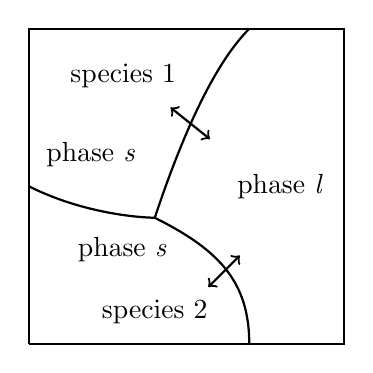
\begin{tikzpicture}[scale=0.4]
    \draw [thick] (0,0) -- (10,0) -- (10,10) -- (0,10) -- (0,0);
    \draw [thick] (0,5) .. controls (2,4) and (4,4) .. (4,4);
    \draw [thick] (4,4) .. controls (5,7) and (6,9) .. (7,10);
    \draw [thick] (4,4) .. controls (6,3) and (7,2) .. (7,0);
    
    %\draw (4,1) node {$\rho_2=c_{2,2}$};
    %\draw (3,8.5) node {$\rho_1=c_{1,1}=c_s$};
    %\draw (7.5,6) node {$c_{1,f}=c_{f}$};
    %\draw (7.8,3) node {$c_{2,f}$};

    \draw (4,1) node {species 2};
    \draw (3,8.5) node {species 1};

    \draw [thick, <->] (5.7,1.8) -- (6.7,2.8);
    \draw [thick, <->] (4.5,7.5) -- (5.75,6.5);
    %\draw [thick, <->] (7.8,3.8) -- (7.8,5.2);
    
		  \draw (2,6) node {phase \textit{s}};
		  \draw (3,3) node {phase \textit{s}};
		  \draw (8,5) node {phase \textit{l}};
\end{tikzpicture}
\caption{Phases and species in an representative volume element (RVE).\label{fig:RVE}}
\end{figure}
%Within the representative volume element $V$, $\gamma_{i,j}$ represents one quantity of the species $i$ present in
%phase $j$, where $i \in {1,2}$ and $j \in \{s,l\}$. 
The advection-diffusion equation governing transport of the mixture chemical species are solved at each time
step. We track only one species and omit the subscript $i$.
\begin{equation}\label{eq:specietransportsimplified}
\frac{\partial \overline{c}}{\partial t} + \nabla \cdot \big( \overline{ c \mathbf{v}} - \phi \mathcal{D}_{l} \nabla c_l \big) = 0,
\end{equation}
where $\overline{c} = \sum_{j\in \{s,l\}} \phi_j c_{j}$ 
and $\overline{c \mathbf{v}} = \sum_{j\in \{s,l\}} \phi_j c_{j} \mathbf{v}_j$
are the mixture quantities. The diffusion term $\frac{\phi \mathcal{D}_l}{u_0l_0} \nabla c_l$ 
is omitted in this work
due to the fact that the porosity $\phi$ remains small ($\phi \ll 1$) in the partially molten mantle
and the associated diffusivity coefficient $\mathcal{D}_l$
is comparatively negligible ~\cite{GeochemicalConsequence} (on the order of $10^{-10}$ to $10^{-9}$ $m^2/s$). 
Effective velocity for the mixture velocity is applied for the equilibrium transport here:
\begin{equation}\label{eq:definitioneffvel}
\bold{v}_{\text{eff}} = \frac{\phi_l \bold{v}_l + D_i\phi_s \bold{v}_s}{\phi_l + \phi_s D_i},
\end{equation}
where the partition coefficient $D_i = c_{i,s}/c_{i,l}$.
In the no melting regions, where $\phi_l = 0$, we retrieve 
$\mathbf{v}_{\text{eff}} = \mathbf{v}_s$.
Conversely, in the case of melting completely, where $\phi_l = 1$, we obtain
$\mathbf{v}_{\text{eff}} = \mathbf{v}_l$.
Therefore, the definition of effective velocity is well-defined in these two limiting scenarios. 
We rewrite the transport equation~\eqref{eq:specietransportsimplified} with 
effective velocity~\eqref{eq:definitioneffvel} as
\begin{equation}\label{eq:effectivetransportspecie}
		  \frac{\partial C}{\partial t} + 
		  \nabla \cdot \mathbf{v}_{\text{eff}} C 
		  = 0,
\end{equation}
where we rewrite $C = \overline{c}$ for simplicity and drop the diffusion term.

We write the temperature formulation of the enthalpy transport equation under the 
extended Boussinesq approximation in terms of the temperature $T$ and the latent heat $L$ as
\begin{equation}\label{eq:normalizedenthalpy}
		  \frac{\partial \overline{H}}{\partial t} + \nabla \cdot (\overline{\mathbf{v}} T) = 
		  \frac{L}{c_p} \nabla \cdot ((1-\phi) \mathbf{v}_s) + \kappa \nabla^2 T + 
		  \frac{\alpha_\rho}{c_p} T \overline{\mathbf{v}} \cdot \mathbf{g},
\end{equation}
where $c_p$ is the specific heat capacity, $\alpha_\rho$ is thermo expansion coefficient.
$\overline{H} = \overline{\rho h}/\rho c_p = \overline{h}/c_p$ is the bulk specific enthalpy and $\kappa = 
\overline{K}/\rho c_p$ is the bulk heat diffusivity.
The last term involving gravitational acceleration is referred 
to as adiabatic cooling or decompression cooling term 
~\cite{ExtensionofLithosphere}.

\subsection{Phase Model}
With the transport equations specified, we are now able to update the distribution of 
chemical species and energy within the system.
The thermodynamic state is then determined under the assumption of local 
thermodynamic equilibrium at each time step.

Given that mid-ocean ridges develop in relatively low-temperature mantle environments, 
eutectic melting provides an appropriate conceptual framework for modeling phase transitions.
In particular, the presence of a secondary component depresses the melting temperature
of the mixture in the binary eutectic model.

%The binary eutectic system has been widely applied in studies involving
%chemical equilibrium.
%%Not only in the context of mantle dynamics~\cite{GenerationCompositionPartialMelts}
%but also in the solidification of 
%alloys~\cite{eutecticsolidification} and in the water-salt-brine systems in glaciers 
%~\cite{DownwardOxidantTransport}. 

The binary eutectic system has been widely employed in studies of chemical equilibrium across a 
range of geophysical and materials science applications. In mantle dynamics, it provides a tractable 
framework for modeling multicomponent melting processes~\cite{GenerationCompositionPartialMelts}. 
Similar formulations have been used to describe alloy solidification in the alloy 
systems~\cite{eutecticsolidification}, 
as well as phase behavior in water–salt–brine systems in glaciers~\cite{DownwardOxidantTransport}.

%We assume the two primary components in our partially molten system are olivine and orthopyroxene (opx), 
%which are highly miscible in the liquid phase, but immiscible in the solid phase.
%Olivine is considered to dominate the system, while orthopyroxene is the 
%minor component.
We consider a partially molten system composed of two primary components: Olivine and Orthopyroxene (opx). 
These components are assumed to be highly miscible in the liquid phase but immiscible in the solid phase. 
Olivine constitutes the dominant component of the system, whereas orthopyroxene represents the minor component.
In this work, we track the concentration of the minor component orthopyroxene.
\begin{figure}[htb]
\centering

\includegraphics[width=10cm,height=7cm]{chapters/pics/eutectic.png}
\caption{Eutectic phase diagram of a Olivine-Orthopyroxene system.}
\label{fig:fullphasediagram}
\end{figure}
A typical eutectic phase diagram is shown in Figure~\ref{fig:fullphasediagram}.
There are two key concepts about the diagram:
\begin{itemize}
\item The eutectic melting point or eutectic temperature $T_e$, represents the minimum temperature
at which melting may occur in this binary system. Melting that takes place at the eutectic temperature 
is referred to as the 
eutectic melting. The temperature of the system is fixed at the eutectic temperature when 
eutectic melting happens.
%\item The eutectic composition $C_e$ is a fixed opx-olivine concentration ratio of the liquid
%produced by eutectic melting.
\item The eutectic bulk composition, $C_e$ corresponds to the fixed orthopyroxene–olivine concentration 
		  ratio of the liquid generated during the eutectic melting. This composition is uniquely determined 
			 by the mixture system and remains constant as long as melting occurs at the eutectic temperature.
\end{itemize}

Pressure can undergo significant variations during 
dynamic events such as mantle upwelling. As a result, the influence of 
pressure on the melting point cannot be neglected.
To account for this, we approximate the solidus melting temperature $T_m$
and the eutectic melting temperature $T_e$
at a given pressure using the approximated Clausius–Clapeyron relationship.
\begin{equation}\label{eq:calusiusclapeyron}
\begin{aligned}
		  T_m &= T_{m0} + \nu^{-1} (P-P_0), \\
		  T_e &= T_{e0} + \nu^{-1} (P-P_0), \\
\end{aligned}
\end{equation}
where $\nu$ is the Clausius-Clapeyron constant, and
$P_0$ is the reference pressure usually set to be 0.
The melting point $T_{m0}$ and eutectic point $T_{e0}$ 
refer to their respective values at standard atmospheric pressure.

%Binary eutectic melting is usually highly-nonlinear.
%For simplicity, we adopt a geometric parameterization of the binary 
%eutectic diagram that can be analytically evaluated. 
%We implement a linear eutectic phase boundary to distinguish between different
%phase regions within the diagram.

Binary eutectic melting is usually highly-nonlinear due to the strong coupling between temperature, 
composition, and phase proportions. To simplify the analysis, we adopt a geometric parameterization of 
the binary eutectic phase diagram that permits analytical evaluation. In particular, we approximate the 
eutectic phase boundaries using linear relations, thereby enabling a clear distinction among the different phase regions and easy phase split calculation.

The eutectic composition of opx is set as $C_e \approx 0.25$. For illustration only, we plot bulk 
composition against a renormalized dimensionless temperature $\check{T} - T_e/\Delta T$, 
where $\check{T}_m - T_e/\Delta T = 1$ and $\check{T}_e - T_e/\Delta T = 0$.
\begin{figure}[htb]
\centering

\includegraphics[width=10cm,height=7cm]{chapters/pics/zoom_eutectic.png}
\caption{
Phase diagram when the composition of opx is smaller than the eutectic composition. Region V does not appear.}
\label{fig:phase_zoom}
\end{figure}

We identify the following $6$ regions with different phase assemblages:
\begin{enumerate}
\item Single-phase sub-solidus    \hspace{0.55cm}: Olivine;
\item Two-phase sub-solidus       \hspace{0.85cm}: Olivine + Orthopyroxene;
\item Three-phase eutectic        \hspace{1.15cm}: Olivine + Orthopyroxene + melt;
\item Two-phase super-eutectic    \hspace{0.3cm}: Olivine + melt;
\item Two-phase super-eutectic    \hspace{0.3cm}: Orthopyroxene + melt;
\item Single-phase super-liquidus : melt.
\end{enumerate}

In the partially molten system considered here, 
the bulk composition of orthopyroxene (opx) is assumed to remain below the eutectic composition.
Consequently, our analysis is restricted to the region of the phase diagram 
Figure~\ref{fig:fullphasediagram}, where the bulk composition is
less than the eutectic composition, which is highlighted in the Figure~\ref{fig:phase_zoom}.

%Melting in the eutectic system is illustrated with the green line in the Figure~\ref{fig:phase_zoom}.
%Now imagining a system containing $17\%$ opx that starts melting. Starting with all solid phase at
%Point $a$, the 
%system temperature increase linearly in response to the enthalpy rise. When the temperature reaches the 
%eutectic temperature, at Point $b$, both components of the system start melting 
%with a fixed ratio of $25\%$ opx and $75\%$ olivine, which is the eutectic composition.
%Once all the solid phase opx is exhausted, the system leaves the eutectic points and solid olivine starts melting.
%The system climbs up along the line from Point $3$
%to Point $c$. After the remaining solid olivine has melted, the temperature of the system will continue to rise linearly
%in response to enthalpy input. It is worth noting that we can reverse the process to obtain a path 
%of equilibrium crystallization.
Melting in the eutectic system is illustrated by the green trajectory in the Figure~\ref{fig:phase_zoom}.Consider a representative system with a bulk composition of $17\%$ orthopyroxene (opx) that undergoes progressive 
heating. Initially, the system is entirely solid (Point a), and its temperature increases 
linearly with increasing enthalpy. 

When the temperature reaches the eutectic temperature (Point b), eutectic melting begins. At this stage, 
both components melt simultaneously in a fixed proportion corresponding to the eutectic composition 
($25\%$ opx and $75\%$ olivine). The temperature remains constant at the eutectic value during this process.

Once all solid opx has been consumed, the system departs from the eutectic point. Further enthalpy input leads
to melting of the remaining solid olivine, and the state evolves along the liquidus line (from Point b toward 
Point c). After complete melting of the residual olivine, the system becomes fully liquid, and the temperature
again increases approximately linearly with additional enthalpy.

The melting path described above is reversible under equilibrium conditions, yielding the corresponding 
trajectory for equilibrium crystallization.

\newpage
\subsection{Parameters}

\begin{table}[ht]
		  \centering\scalebox{1.3}{
\begin{tabular}{c | c c}
Quantity & Value & Units \\
\hline
%$\rho$       & $3000$           & $kg\cdot m^{-3}$              \\
%$\rho_r$       & $600$           & $kg\cdot m^{-3}$              \\
%$\alpha_\rho$  & $3\times10^{-5}$ & $K^{-1}$                      \\
%$c_p$          & $1200$           & $J\cdot kg^{-1} \cdot K^{-1}$ \\
%$L$            & $5\times10^{5}$  & $J\cdot kg^{-1}$              \\
%$\mu_l$        & $1$              & $\text{Pascal} \cdot s$       \\
%$\mu_s$        & $10^{19}$        & $\text{Pascal} \cdot s$       \\
%$k_0$          & $10^{-8}$        & $m^2$                         \\
%$T_{e0}$       & $1480$           & $K$                           \\
%$T_{m0}$       & $2000$           & $K$                           \\
%$\nu$          & $6.5\times10^6$  & $\text{Pascal} \cdot K^{-1}$
		  $\rho$       & $3000$           & $\text{kg}\cdot \text{m}^{-3}$              \\
		  $\rho_r$       & $600$           & $\text{kg}\cdot \text{m}^{-3}$              \\
		  $\alpha_\rho$  & $3\times10^{-5}$ & $\text{K}^{-1}$                      \\
		  $c_p$          & $1200$           & $\text{J}\cdot \text{kg}^{-1} \cdot \text{K}^{-1}$ \\
		  $L$            & $5\times10^{5}$  & $\text{J}\cdot \text{kg}^{-1}$              \\
		  $\mu_l$        & $1$              & $\text{Pascal} \cdot \text{s}$       \\
		  $\mu_s$        & $10^{19}$        & $\text{Pascal} \cdot \text{s}$       \\
		  $k_0$          & $10^{-8}$        & $\text{m}^2$                         \\
		  $T_{e0}$       & $1480$           & $\text{K}$                           \\
		  $T_{m0}$       & $2000$           & $\text{K}$                           \\
		  $\nu$          & $6.5\times10^6$  & $\text{Pascal} \cdot \text{K}^{-1}$
\end{tabular}}
\caption[Parameters Table]{Flow Mechanics and Thermodynamics Parameters}
\label{tab:parameters}
\end{table}
